\chapter{End-to-End Machine Learning Project\label{End-to-End Machine Learning Project}}
\section{Working with Real Data\label{Working with Real Data}}

When you are learning about Machine Learning, it is best to experiment with realworld data, not artificial datasets. Here are a few places you can look
to get data:
\begin{itemize}
\item Popular open data repositories
\begin{itemize}
\item \href{http://archive.ics.uci.edu/ml/index.php}{UC Irvine Machine Learning Repository}

\item \href{https://www.kaggle.com/datasets}{Kaggle datasets}

\item \href{https://registry.opendata.aws/}{Amazon’s AWS datasets}
\end{itemize}

\item Meta portals (they list open data repositories)
\begin{itemize}
\item \href{http://dataportals.org/}{Data Portals}

\item \href{http://opendatamonitor.eu/}{OpenDataMonitor}

\item \href{https://data.nasdaq.com/}{Quandl}
\end{itemize}

\item Other pages listing many popular open data repositories
\begin{itemize}
\item \href{https://en.wikipedia.org/wiki/List_of_datasets_for_machine-learning_research}{Wikipedia’s list of Machine Learning datasets}

\item\href{https://www.quora.com/Where-can-I-find-large-datasets-open-to-the-public}{Quora.com}

\item\href{https://www.reddit.com/r/datasets/}{The datasets subreddit}
\end{itemize}
\end{itemize}

\section{Look at the Big Picture}
\subsection{Frame the Problem}
The first question to ask your boss is what exactly the business objective is. Building a
model is probably not the end goal. How does the company expect to use and benefit
from this model? Knowing the objective is important because it will determine how
you frame the problem, which algorithms you will select, which performance measure you will use to evaluate your model, and how much effort you will spend tweaking it.

Your boss answers that your model’s output (a prediction of a district’s median housing price) will be fed to another Machine Learning system (see \autoref{A Machine Learning pipeline for real estate investments}), along
with many other signals\footnote{A piece of information fed to a Machine Learning system is often called a signal, in reference to Claude Shannon’s information theory, which he developed at Bell Labs to improve telecommunications. His theory: you
want a high signal-to-noise ratio.}.

\begin{figure}
\centering
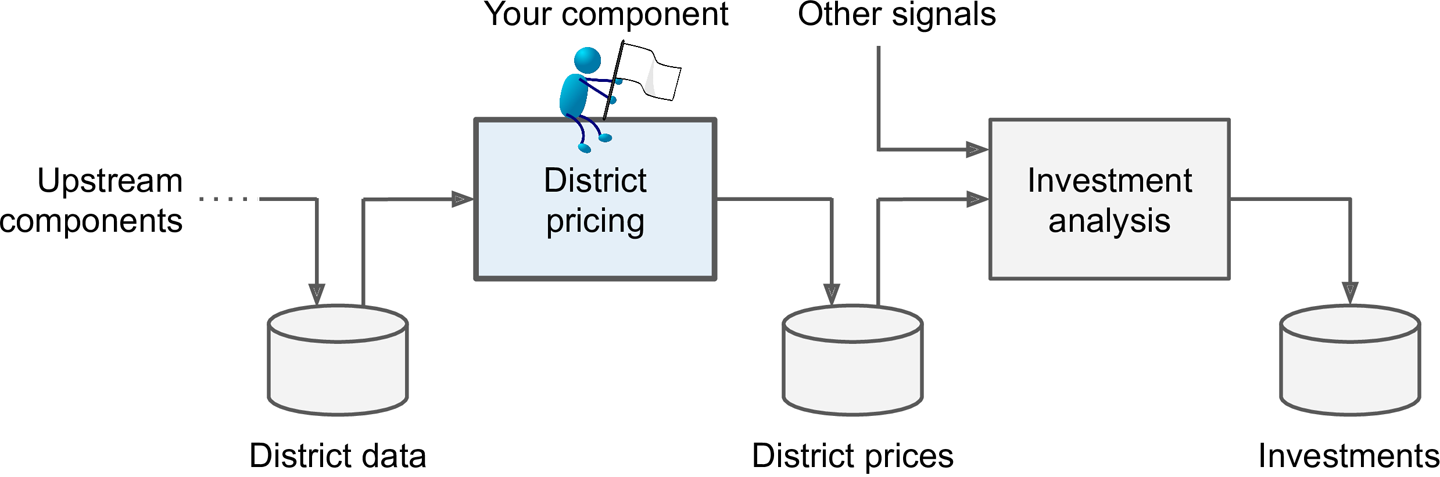
\includegraphics{img/A Machine Learning pipeline for real estate investments.png}
\caption{A Machine Learning pipeline for real estate investments}
\label{A Machine Learning pipeline for real estate investments}
\end{figure}
\explain{Pipelines}{
A sequence of data processing components is called a data pipeline. Pipelines are very
common in Machine Learning systems, since there is a lot of data to manipulate and
many data transformations to apply.

Components typically run asynchronously. Each component pulls in a large amount
of data, processes it, and spits out the result in another data store. Then, some time
later, the next component in the pipeline pulls this data and spits out its own output.
Each component is fairly self-contained: the interface between components is simply
the data store. This makes the system simple to grasp (with the help of a data flow
graph), and different teams can focus on different components. Moreover, if a component breaks down, the downstream components can often continue to run normally (at least for a while) by just using the last output from the broken component.
This makes the architecture quite robust.

On the other hand, a broken component can go unnoticed for some time if proper
monitoring is not implemented. The data gets stale and the overall system’s performance drops.
}

The next question to ask your boss is what the current solution looks like (if any).
The current situation will often give you a reference for performance

\textbf{Tips:}If the data were huge, you could either split your batch learning
work across multiple servers (using the MapReduce technique) or
use an online learning technique.

\subsection{Select a Performance Measure}
Your next step is to select a performance measure. A typical performance measure for
regression problems is the Root Mean Square Error (RMSE). It gives an idea of how
much error the system typically makes in its predictions, with a higher weight for
large errors. \autoref{RMSE} shows the mathematical formula to compute the RMSE.

\begin{equation}\label{RMSE}
RMSE(\mathbf{X}, h) = \sqrt{\frac{1}{m}\sum_{i=1}^m(h(x^{(i)})-y^{(i)})^2}
\end{equation}

\explain{Notations}{
This equation introduces several very common Machine Learning notations that we
will use throughout this book:
\begin{itemize}
\item $m$ is the number of instances in the dataset you are measuring the RMSE on.

\item $\mathbf{x}^{(i)}$ is a vector of all the feature values (excluding the label) of the $i^{th}$ instance in
the dataset, and $y^{(i)}$ is its label (the desired output value for that instance). e.g., 
\begin{align*}
\mathbf{x}^{(i)}&=\begin{bmatrix}
-118.29\\
33.91\\
1,416\\
38,372
\end{bmatrix}
\end{align*}


\item
$\mathbf{X}$ is a matrix containing all the feature values (excluding labels) of all instances in
the dataset. There is one row per instance, and the $i^{th}$ row is equal to the transpose of $\mathbf{x}^{(i)}$, noted $(\mathbf{x}^{(i)})^T$. e.g.,

\begin{align*}
\mathbf{x}^{(i)}&=\begin{bmatrix}
(\mathbf{x}^{(1)})^T\\
(\mathbf{x}^{(2)})^T\\
\vdots\\
(\mathbf{x}^{(m-1)})^T\\
(\mathbf{x}^{(m)})^T
\end{bmatrix}=\begin{bmatrix}
-118.29&33.91&1,416&38,372\\
\vdots&\vdots&\vdots&\vdots\\
\end{bmatrix}
\end{align*}
\item  $h$ is your system’s prediction function, also called a \emph{hypothesis}. When your system
is given an instance’s feature vector $\mathbf{x}^{(i)}$, it outputs a predicted value $\hat{y}^{(i)} = h(\mathbf{x}^{(i)})$ for that instance.

\item $RMSE(\mathbf{X}, h)$ is the cost function measured on the set of examples using your
hypothesis \emph{h}.

We use lowercase italic font for scalar values and function names, lowercase bold font for vectors, and uppercase bold font for
matrices.
\end{itemize}
}

Even though the RMSE is generally the preferred performance measure for regression
tasks, in some contexts you may prefer to use another function. For example, \textbf{suppose
that there are many outlier districts. In that case, you may consider using the mean
absolute error} (MAE, also called the average absolute deviation; see \autoref{MAE}):

\begin{equation}\label{MAE}
MAE(\mathbf{X}, h) = \frac{1}{m}\sum_{i=1}^m|h(x^{(i)})-y^{(i)}|
\end{equation}

Both the RMSE and the MAE are ways to measure the distance between two vectors:
the vector of predictions and the vector of target values. Various distance measures,
or \emph{norms}, are possible:

\begin{itemize}
\item
Computing the root of a sum of squares (RMSE) corresponds to the \emph{Euclidean
norm}: this is the notion of distance you are familiar with. It is also called the \emph{$l_2$
norm}, noted $||\cdot||_2$ (or just$||\cdot||$).
\item
Computing the sum of absolutes (MAE) corresponds to the \emph{$l_1$ norm}, noted $||\cdot||_1$.
This is sometimes called the \emph{Manhattan norm} because it measures the distance
between two points in a city if you can only travel along orthogonal city blocks.
\item More generally, the $l_k$ norm of a vector $v$ containing $n$ elements is defined as $||v||_k
= (|v_0|^k + |v_1|^k + \cdots + |v_n|^k)^{1/k}$. $l_0$ gives the number of nonzero elements in the vector, and $l_\infty$ gives the maximum absolute value in the vector.
\item \textbf{The higher the norm index, the more it focuses on large values and neglects small
ones.} This is why the RMSE is more sensitive to outliers than the MAE. But when
outliers are exponentially rare (like in a bell-shaped curve), the RMSE performs
very well and is generally preferred.
\end{itemize}

\subsection{Check the Assumptions}
Lastly, it is good practice to list and verify the assumptions that have been made so far
(by you or others); this can help you catch serious issues early on. For example, the
district prices that your system outputs are going to be fed into a downstream
Machine Learning system, and you assume that these prices are going to be used as
such. But what if the downstream system converts the prices into categories (e.g.,
“cheap,” “medium,” or “expensive”) and then uses those categories instead of the pri‐
ces themselves? In this case, getting the price perfectly right is not important at all;
your system just needs to get the category right. If that’s so, then the problem should
have been framed as a classification task, not a regression task. You don’t want to find
this out after working on a regression system for months.

\section{Get the Data}
The full Jupyter notebook is available at \url{https://github.com/JPL-JUNO/HOML}.
\subsection{Create the Workspace}
You will need to have Python installed. It is probably already installed on your
system. If not, you can get it at \url{https://www.python.org/}.

If you already have Jupyter running with all these modules installed,
you can safely skip to \nameref{Download the Data}.
\subsection{Download the Data\label{Download the Data}}

Having a function that downloads the data is useful in particular if the
data changes regularly: you can write a small script that uses the function to fetch the
latest data (or you can set up a scheduled job to do that automatically at regular intervals). Automating the process of fetching the data is also useful if you need to install
the dataset on multiple machines.

\subsection{Take a Quick Look at the Data Structure}
Let’s take a look at the five rows using the DataFrame’s \verb|sample(n=5)| method instead of \verb|head(n=5)|.

The \verb|info()| method is useful to get a quick description of the data, in particular the
total number of rows, each attribute’s type, and the number of nonnull values. Notice that the 
\verb|total_bedrooms| attribute has only 20,433 nonnull values, meaning that 207 districts are missing
this feature. We will need to take care of this later.

You can find out what cate‐
gories exist and how many districts belong to each category by using the
\verb|value_counts()| method:

\begin{minted}{python}
housing['ocean_proximity'].value_counts()
\end{minted}

The \verb|describe()| method shows a summary of the
numerical attributes. When with many columns, you can use \verb|transpose()| for best information.
\begin{minted}{python}
# housing.describe()
housing.describe().transpose()
\end{minted}


